\documentclass[12pt,a4paper]{article}
\usepackage{amsmath,amsthm,amssymb,mathtools}
\usepackage{tikz}
\usetikzlibrary{arrows.meta,positioning,shapes.geometric,calc,fit,backgrounds}
\usepackage{graphicx}
\usepackage{booktabs,tabularx,multirow}
\usepackage[ruled,vlined,linesnumbered]{algorithm2e}
\usepackage[most]{tcolorbox}
\usepackage{hyperref}
\usepackage[capitalize,noabbrev]{cleveref}
\usepackage[margin=1in]{geometry}
\usepackage{fancyhdr}
\usepackage{enumitem}
\usepackage{xcolor}

%% ── tcolorbox environments ──────────────────────────────────────────────────
\newtcolorbox{keyinsight}[1][]{colback=blue!5!white,colframe=blue!75!black,fonttitle=\bfseries,title=Key Insight,#1}
\newtcolorbox{example}[1][]{colback=green!5!white,colframe=green!75!black,fonttitle=\bfseries,title=Example,#1}
\newtcolorbox{warningbox}[1][]{colback=red!5!white,colframe=red!75!black,fonttitle=\bfseries,title=Warning,#1}

%% ── amsthm environments ─────────────────────────────────────────────────────
\newtheorem{theorem}{Theorem}[section]
\newtheorem{lemma}[theorem]{Lemma}
\newtheorem{definition}{Definition}[section]
\newtheorem{remark}{Remark}[section]

%% ── Header / footer ─────────────────────────────────────────────────────────
\pagestyle{fancy}
\fancyhf{}
\rhead{Deep Learning -- Session 20}
\lhead{LSTM Numerical Walkthrough \& Next-Word Prediction}
\cfoot{\thepage}

%% ── Hyperref setup ──────────────────────────────────────────────────────────
\hypersetup{
  colorlinks=true,
  linkcolor=blue!70!black,
  urlcolor=blue!70!black,
  citecolor=green!50!black
}

%% ── Convenience macros ──────────────────────────────────────────────────────
\newcommand{\sigmoid}{\sigma}
\newcommand{\R}{\mathbb{R}}
\newcommand{\odotop}{\odot}

\begin{document}

%% ============================================================
%%  TITLE PAGE
%% ============================================================
\begin{titlepage}
  \centering
  \vspace*{2cm}
  {\LARGE\bfseries Deep Learning: Course Notes\par}
  \vspace{0.8cm}
  \rule{\linewidth}{0.5pt}\\[0.4cm]
  {\huge\bfseries Session 20\\[0.3cm]
   LSTM Numerical Walkthrough\\[0.2cm]
   \& Next-Word Prediction Hands-On\par}
  \rule{\linewidth}{0.5pt}\\[1.5cm]

  \begin{tabular}{rl}
    \textbf{Session Number:} & 20 \\[4pt]
    \textbf{Date:}           & January 31, 2026 \\[4pt]
    \textbf{Instructors:}    & Prof.\ S.\ R.\ M.\ Prasanna \\
                             & Dr.\ Sunil Saumya \\[4pt]
    \textbf{Institute:}      & IIIT Dharwad \\[4pt]
    \textbf{Slide Deck:}     & \texttt{05-DL-RNN} (slides 35, 39, 42 of 75) \\[4pt]
    \textbf{Video:}          & \url{https://vimeo.com/1160427634} \\[4pt]
    \textbf{Duration:}       & $\approx 1$ hr 41 min \\
  \end{tabular}

  \vfill
  {\large\itshape Topics Covered}\\[0.4cm]
  \begin{itemize}[leftmargin=4cm,rightmargin=4cm]
    \item LSTM recurrence cell recap (Colah's blog style diagram)
    \item Forget Gate -- detailed numerical walkthrough
    \item Input Gate -- sigmoid and tanh sub-operations
    \item Output Gate -- filtered memory exposure
    \item Cell-state update equation
    \item GRU comparison (brief)
    \item Hands-on: next-word prediction with PyTorch LSTM
    \item Pre-processing pipeline: tokenisation, vocabulary, sliding-window sequences, padding
    \item \texttt{LSTMModel} class implementation
  \end{itemize}
  \vfill
\end{titlepage}

\tableofcontents
\newpage

%% ============================================================
\section{Introduction}
\label{sec:intro}
%% ============================================================

Session 20 of the deep learning course is devoted to two complementary goals.
The first half provides a careful, \emph{numerical} walkthrough of how the three
gates of a Long Short-Term Memory (LSTM) cell operate, working with explicit
4-dimensional vectors so that every dot-product, sigmoid evaluation, and
element-wise multiplication can be traced by hand.
The second half transitions to a fully working hands-on session in which an
LSTM is trained to perform \emph{next-word prediction} on a short text corpus,
walking through every stage of the PyTorch pipeline: tokenisation, vocabulary
construction, self-supervised sequence creation, padding, custom dataset and
data loader, model definition, and training.

\begin{keyinsight}
  The central motivation for LSTM is the \emph{vanishing gradient} problem of
  vanilla RNNs.  A plain RNN uses a \emph{single} hidden-state vector that must
  simultaneously encode short-term context (the current word) and long-term
  context (words seen many steps ago).  As back-propagation is applied through
  many time steps, gradients shrink exponentially, making it practically
  impossible to learn long-range dependencies.
  LSTM introduces a dedicated \textbf{cell state} $C_t$ that acts as a
  long-term memory highway, updated only through controlled additive operations
  that let gradients flow almost unchanged across many time steps.
\end{keyinsight}

The session is taught by Dr.\ Sunil Saumya (theoretical portion) and references
Prof.\ S.\ R.\ M.\ Prasanna's slides from the \texttt{05-DL-RNN} deck.
The visual material is drawn from Christopher Olah's widely cited blog post
``Understanding LSTM Networks'' (2015), which provides the iconic cell-diagram
used throughout the lecture.

%% ============================================================
\section{Background and Prerequisites}
\label{sec:background}
%% ============================================================

\subsection{Vanilla RNN and Its Limitations}
\label{subsec:rnn-limits}

A standard (Elman) RNN maintains a single hidden state $h_t$ updated as

\begin{equation}
  h_t = \tanh\!\bigl(W_h h_{t-1} + W_x x_t + b\bigr),
  \label{eq:rnn-update}
\end{equation}

where $x_t \in \R^d$ is the input at time step $t$, $W_h$ and $W_x$ are
learned weight matrices, and $b$ is a bias vector.
The same vector $h_t$ serves as both:
\begin{itemize}
  \item the \textbf{short-term} representation passed forward to the next cell, and
  \item the \textbf{long-term} carrier of all contextual information seen so far.
\end{itemize}
Because $h_t$ is overwritten at every step, information from distant time steps
(e.g.\ $x_{100}$) is diluted by the time the network processes $x_1$ in
reverse during BPTT, resulting in near-zero gradients --- the vanishing
gradient problem.

\subsection{Word Representations}
\label{subsec:word-rep}

Before feeding text into any recurrent network, words must be converted to
vectors.  Two representations are used in this session:

\begin{description}[style=nextline]
  \item[One-hot vectors] A vocabulary of size $V$ maps each word to a binary
    vector $v \in \{0,1\}^V$ with exactly one non-zero entry.  This is
    sparse, high-dimensional, and carries no semantic information.
  \item[Dense embeddings] An \texttt{nn.Embedding} layer learns a weight matrix
    $E \in \R^{V \times d_e}$; look-up of word index $i$ returns the $i$-th
    row, producing a dense $d_e$-dimensional vector.  This dramatically reduces
    dimensionality and allows the network to learn semantic similarity.
\end{description}

\begin{remark}
  In the running example used during the lecture, the vocabulary contains
  $V = 4$ words (\emph{I}, \emph{love}, \emph{deep}, \emph{learning}) and the
  embedding dimension is set to $d_e = 4$, giving equal embedding and hidden
  dimensions for simplicity.  In the later hands-on, $V = 289$, $d_e = 100$.
\end{remark}

\subsection{Tensor Dimensions for LSTM Input}
\label{subsec:tensor-dims}

With \texttt{batch\_first=True} (PyTorch convention used in this session),
the input tensor has shape

\[
  \text{input} \;\in\; \R^{B \times T \times d_e},
\]

where $B$ is the batch size, $T$ is the sequence length (number of time steps),
and $d_e$ is the embedding dimension.  For the minimal toy example
($B=1$, $T=4$, $d_e=4$) the shape is $1 \times 4 \times 4$.

%% ============================================================
\section{LSTM Cell Architecture}
\label{sec:lstm-arch}
%% ============================================================

\subsection{The Two-Stream Design}
\label{subsec:two-stream}

The defining architectural choice of an LSTM is the separation of internal
memory into two distinct vectors:

\begin{itemize}
  \item \textbf{Cell state} $C_t \in \R^H$ --- the long-term memory highway.
    It flows from left to right across the unrolled cell with only two
    point-wise operations (one multiplication and one addition), so gradients
    can propagate almost unchanged over many steps.
  \item \textbf{Hidden state} $h_t \in \R^H$ --- the short-term, context-filtered
    output.  It is derived from $C_t$ at each step and is what the cell exposes
    to the next time step and to downstream layers.
\end{itemize}

\begin{keyinsight}[title=Memory Storage vs.\ Memory Exposure]
  The instructor uses an evocative analogy: think of $C_t$ as everything stored
  in your brain --- childhood memories, professional knowledge, personal plans
  --- all of which is available but not all simultaneously relevant.  When
  someone asks you about LSTM, you draw on only the relevant subset and
  express it as your answer; that filtered response is $h_t$.
  LSTM explicitly \emph{separates memory storage} ($C_t$) from
  \emph{memory exposure} ($h_t$).
\end{keyinsight}

\subsection{TikZ Diagram: LSTM Recurrence Cell}
\label{subsec:lstm-diagram}

\cref{fig:lstm-cell} recreates the Colah's-blog style cell diagram shown on
slide 35/75 of the lecture deck.

\begin{figure}[ht]
\centering
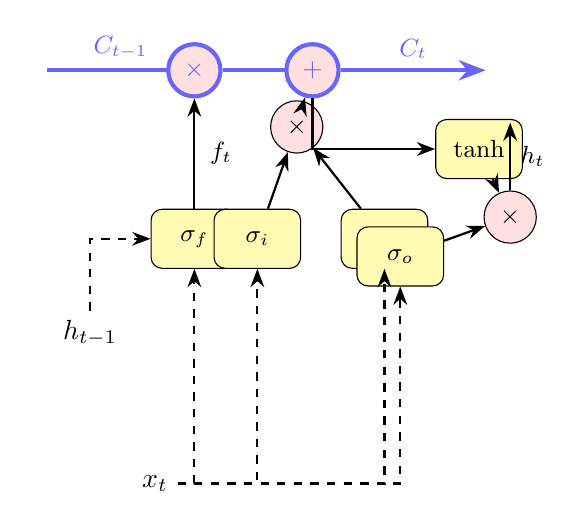
\begin{tikzpicture}[
    >=Stealth,
    node distance=1.3cm and 1.6cm,
    gate/.style={draw, rounded corners=4pt, fill=yellow!30,
                 minimum width=1.1cm, minimum height=0.75cm, font=\small},
    op/.style={draw, circle, fill=pink!50, minimum size=0.55cm, font=\small\bfseries},
    vec/.style={->, thick},
    label/.style={font=\small\itshape}
  ]

  %% Cell state line (top horizontal highway)
  \node (cin)  [left=2.5cm of {(0,1.8)}] {};
  \node (cout) [right=5.8cm of cin]       {};
  \draw[vec, line width=1.5pt, blue!60] (cin) -- node[above, label]{$C_{t-1}$} ++(2.0,0)
       node (cmul) [op] {$\times$};
  \draw[vec, line width=1.5pt, blue!60] (cmul) -- ++(1.5,0)
       node (cadd) [op] {$+$};
  \draw[vec, line width=1.5pt, blue!60] (cadd) -- node[above, label]{$C_t$} ++(2.2,0);

  %% Forget gate
  \node (fg) [gate, below=1.4cm of cmul] {$\sigma_f$};
  \draw[vec] (fg) -- node[right, label, xshift=2pt]{$f_t$} (cmul);

  %% Input gate (sigmoid part)
  \node (ig) [gate, below=1.4cm of cadd, xshift=-0.7cm] {$\sigma_i$};
  %% Candidate (tanh part)
  \node (tg) [gate, right=0.5cm of ig] {$\tanh$};
  %% Multiply i_t and ~C_t
  \node (imul) [op, above=0.7cm of ig, xshift=0.5cm] {$\times$};
  \draw[vec] (ig)  -- (imul);
  \draw[vec] (tg)  -- (imul);
  \draw[vec] (imul) -- (cadd);

  %% Output gate
  \node (tanh2) [gate, right=1.2cm of cadd, yshift=-1.0cm] {$\tanh$};
  \node (og)    [gate, below=0.6cm of tanh2, xshift=-1.0cm] {$\sigma_o$};
  \node (omul)  [op,   right=0.5cm of og, yshift=0.5cm] {$\times$};
  \draw[vec] (cadd)  |- (tanh2);
  \draw[vec] (tanh2) -- (omul);
  \draw[vec] (og)    -- (omul);
  \draw[vec] (omul)  -- node[right, label]{$h_t$} ++(0,1.2);

  %% Input lines for x_t and h_{t-1}
  \node (xt)   [below=2.5cm of fg, xshift=-0.5cm]  {$x_t$};
  \node (htm1) [left=0.3cm of fg, yshift=-1.2cm]   {$h_{t-1}$};
  \draw[vec, dashed] (xt)   -| (fg);
  \draw[vec, dashed] (htm1) |- (fg);
  \draw[vec, dashed] (xt)   -| (ig);
  \draw[vec, dashed] (xt)   -| (tg);
  \draw[vec, dashed] (xt)   -| (og);

\end{tikzpicture}
\caption{LSTM recurrence cell (Colah's blog style, slide 35/75).
  Blue: cell-state highway $C_t$.
  Yellow rectangles: learned single-layer sub-networks (gates).
  Pink circles: point-wise operations ($\times$ = element-wise multiply,
  $+$ = element-wise add).
  The four internal networks are: forget gate ($\sigma_f$), input gate
  ($\sigma_i$), candidate generator ($\tanh$), and output gate ($\sigma_o$).}
\label{fig:lstm-cell}
\end{figure}

%% ============================================================
\section{LSTM Gate Mathematics and Numerical Walkthrough}
\label{sec:gates}
%% ============================================================

This section presents the complete forward-pass equations for one LSTM time
step, followed by the 4-dimensional numerical example worked through by the
instructor.

\subsection{Notation and Setup}
\label{subsec:notation}

Throughout, the LSTM has $H$ hidden units (neurons per gate).  At time step
$t$ the following vectors are available:

\begin{center}
\begin{tabular}{lll}
\toprule
\textbf{Symbol} & \textbf{Shape} & \textbf{Description} \\
\midrule
$x_t$     & $\R^d$  & Input embedding at time $t$ \\
$h_{t-1}$ & $\R^H$  & Hidden state from previous step \\
$C_{t-1}$ & $\R^H$  & Cell state from previous step \\
$f_t$     & $\R^H$  & Forget gate output \\
$i_t$     & $\R^H$  & Input gate output \\
$\tilde{C}_t$ & $\R^H$ & Candidate cell values \\
$o_t$     & $\R^H$  & Output gate \\
$C_t$     & $\R^H$  & Updated cell state \\
$h_t$     & $\R^H$  & Updated hidden state \\
\bottomrule
\end{tabular}
\end{center}

In the lecture example, $d = H = 4$ (4-dimensional vectors throughout).

\subsection{Forget Gate}
\label{subsec:forget-gate}

\begin{definition}[Forget Gate]
  The forget gate $f_t$ is a vector in $[0,1]^H$ computed by a single-layer
  neural network with sigmoid activation.  It decides, for each dimension of
  the cell state, what fraction of $C_{t-1}$ to \emph{retain}.
\end{definition}

\begin{align}
  z_f &= W_{xf}\, x_t + W_{hf}\, h_{t-1} + b_f, \label{eq:zf} \\
  f_t &= \sigma(z_f), \label{eq:ft}
\end{align}

where $W_{xf} \in \R^{H \times d}$, $W_{hf} \in \R^{H \times H}$,
$b_f \in \R^H$.

\textbf{Interpretation.}
Each element $f_t[k] \in [0,1]$:
\begin{itemize}
  \item $f_t[k] \approx 1$: keep almost all of $C_{t-1}[k]$.
  \item $f_t[k] \approx 0$: erase almost all of $C_{t-1}[k]$.
  \item $f_t[k] \in (0,1)$: partial retention (soft gating).
\end{itemize}

The forget-gated cell state is then

\begin{equation}
  C_{t-1}^{\text{forget}} = f_t \odot C_{t-1}.
  \label{eq:forget-applied}
\end{equation}

\subsubsection{Numerical Example (Forget Gate)}
\label{subsubsec:forget-numerical}

\begin{example}[title=Forget Gate -- 4-D Numerical Example (slide 42/75)]
Given:
\[
  x_t = \begin{bmatrix} 0.2 \\ 0.6 \\ 0.1 \\ 0.9 \end{bmatrix},\quad
  h_{t-1} = \begin{bmatrix} 0.5 \\ 0.1 \\ 0.3 \\ 0.7 \end{bmatrix},\quad
  C_{t-1} = \begin{bmatrix} 0.9 \\ 0.2 \\ 0.8 \\ 0.4 \end{bmatrix}.
\]

After applying \cref{eq:zf} with some fixed $W_{xf},W_{hf},b_f$:
\[
  z_f = \begin{bmatrix} 1.2 \\ -0.5 \\ 0.3 \\ 2.0 \end{bmatrix}.
\]

Applying sigmoid element-wise:
\[
  f_t = \sigma(z_f) = \begin{bmatrix}
    \sigma(1.2) \\ \sigma(-0.5) \\ \sigma(0.3) \\ \sigma(2.0)
  \end{bmatrix}
  = \begin{bmatrix} 0.77 \\ 0.38 \\ 0.57 \\ 0.88 \end{bmatrix}.
\]

Element-wise multiplication with $C_{t-1}$ (\cref{eq:forget-applied}):
\[
  f_t \odot C_{t-1}
  = \begin{bmatrix} 0.77 \\ 0.38 \\ 0.57 \\ 0.88 \end{bmatrix}
  \odot
  \begin{bmatrix} 0.9 \\ 0.2 \\ 0.8 \\ 0.4 \end{bmatrix}
  = \begin{bmatrix} 0.69 \\ 0.08 \\ 0.46 \\ 0.35 \end{bmatrix}.
\]

\textbf{Reading off the result:}
\begin{itemize}
  \item Dimension 0: 77\% of 0.9 retained $\to$ 0.69 (moderate forgetting).
  \item Dimension 1: only 38\% of 0.2 retained $\to$ 0.08 (mostly forgotten).
  \item Dimension 2: 57\% of 0.8 retained $\to$ 0.46 (partial forgetting).
  \item Dimension 3: 88\% of 0.4 retained $\to$ 0.35 (mostly kept).
\end{itemize}
\end{example}

\subsection{Input Gate and Candidate Cell State}
\label{subsec:input-gate}

The input gate has \emph{two} sub-components operating in parallel:

\begin{align}
  i_t         &= \sigma\!\bigl(W_{xi}\,x_t + W_{hi}\,h_{t-1} + b_i\bigr),
                \label{eq:it} \\
  \tilde{C}_t &= \tanh\!\bigl(W_{xC}\,x_t + W_{hC}\,h_{t-1} + b_C\bigr).
                \label{eq:Ct-cand}
\end{align}

\begin{description}
  \item[$\tilde{C}_t$ (candidate cell).] The $\tanh$ layer generates new
    \emph{candidate values} in $[-1,1]^H$ --- what new information \emph{could}
    be added to memory based on the current context.
  \item[$i_t$ (input gate).] The sigmoid layer decides, for each dimension,
    \emph{how much} of the candidate to actually write into memory.
\end{description}

\begin{keyinsight}[title=Analogy for Input Gate]
  Imagine learning that ``deep learning is a subfield of machine learning.''
  The candidate $\tilde{C}_t$ represents \emph{all} the new information
  (everything about deep learning).  The input gate $i_t$ decides that you
  should add only \emph{part} of it --- perhaps already knowing machine
  learning means the overlap can be discarded.
  So the actual addition to memory is $i_t \odot \tilde{C}_t$: only
  the fraction $i_t[k]$ of each candidate dimension is written.
\end{keyinsight}

\subsection{Cell State Update}
\label{subsec:cell-update}

The new cell state combines the forget-gated old memory with the input-gated
new information:

\begin{equation}
  \boxed{C_t = f_t \odot C_{t-1} \;+\; i_t \odot \tilde{C}_t.}
  \label{eq:cell-update}
\end{equation}

This is the core LSTM update equation.  Crucially, it is purely
\emph{additive}: information is subtracted (via multiplication by $f_t < 1$)
or added (via $i_t \odot \tilde{C}_t$), but there is no tanh squashing of the
highway itself, which is what allows gradients to flow far back in time.

\subsection{Output Gate and Hidden State}
\label{subsec:output-gate}

Finally, the output gate decides what part of the (now-updated) cell state
to expose as the hidden state:

\begin{align}
  o_t &= \sigma\!\bigl(W_{xo}\,x_t + W_{ho}\,h_{t-1} + b_o\bigr),
         \label{eq:ot} \\
  h_t &= o_t \odot \tanh(C_t).
         \label{eq:ht}
\end{align}

The $\tanh(C_t)$ squashes cell-state values into $[-1,1]$, and $o_t$ acts as
a soft mask that selects which dimensions are relevant for the current output.

\begin{remark}
  A student question during the lecture highlighted that all three sigmoid
  outputs ($f_t$, $i_t$, $o_t$) share the same functional form
  (linear combination followed by sigmoid) and even the same inputs
  ($x_t$ and $h_{t-1}$).  What distinguishes them are:
  (1) separate weight matrices ($W_{*f}$, $W_{*i}$, $W_{*o}$) that are
  independently learned; and
  (2) the object each gate is \emph{applied to}: $f_t$ acts on $C_{t-1}$,
  $i_t$ acts on the candidate $\tilde{C}_t$, and $o_t$ acts on $\tanh(C_t)$.
\end{remark}

\subsection{Complete LSTM Forward-Pass Summary}
\label{subsec:full-pass}

Collecting \cref{eq:ft,eq:it,eq:Ct-cand,eq:cell-update,eq:ot,eq:ht}:

\begin{align}
  f_t         &= \sigma(W_{xf}x_t + W_{hf}h_{t-1} + b_f) \label{eq:full-ft} \\
  i_t         &= \sigma(W_{xi}x_t + W_{hi}h_{t-1} + b_i) \label{eq:full-it} \\
  \tilde{C}_t &= \tanh(W_{xC}x_t + W_{hC}h_{t-1} + b_C) \label{eq:full-Ct} \\
  C_t         &= f_t \odot C_{t-1} + i_t \odot \tilde{C}_t \label{eq:full-cell} \\
  o_t         &= \sigma(W_{xo}x_t + W_{ho}h_{t-1} + b_o) \label{eq:full-ot} \\
  h_t         &= o_t \odot \tanh(C_t) \label{eq:full-ht}
\end{align}

\subsection{Dimensional Consistency Constraint}
\label{subsec:dim-constraint}

A key point stressed by the instructor: all gate outputs, the cell state,
and the hidden state must share the same dimension $H$.  This is enforced by
the number of neurons in each gate sub-network.

\begin{warningbox}[title=Dimension Mismatch Will Break the Forward Pass]
  If you set the number of neurons to $H' \neq H$, the gate outputs will be
  $\R^{H'}$-vectors while $C_{t-1} \in \R^H$.  The element-wise operations
  in \cref{eq:forget-applied,eq:cell-update} require identical shapes, so
  PyTorch will raise a dimension mismatch error.  PyTorch's \texttt{nn.LSTM}
  enforces this automatically via its \texttt{hidden\_size} parameter.
\end{warningbox}

\subsection{Gate Parameter Count}
\label{subsec:param-count}

For a single LSTM layer with input dimension $d$ and hidden size $H$,
the total number of trainable parameters is:

\begin{equation}
  \text{Params}_{\text{LSTM}} = 4 \times \bigl(H \cdot d + H \cdot H + H\bigr)
  = 4H(d + H + 1).
  \label{eq:param-count}
\end{equation}

The factor of 4 comes from the four sub-networks: forget gate, input gate,
candidate generator, and output gate.

\begin{example}[title=Parameter Count for the Hands-On Model]
  With $d = 100$ (embedding dimension) and $H = 150$ (hidden size):
  \[
    \text{Params}_{\text{LSTM}} = 4 \times 150 \times (100 + 150 + 1)
    = 600 \times 251 = 150\,600.
  \]
\end{example}

\newpage
\subsection{LSTM Algorithm}
\label{subsec:algorithm}

\begin{algorithm}[H]
\SetAlgoLined
\linesnumbered
\DontPrintSemicolon
\caption{LSTM Single Time-Step Forward Pass}
\label{alg:lstm-forward}
\KwIn{$x_t \in \R^d$, $h_{t-1} \in \R^H$, $C_{t-1} \in \R^H$,
      weight matrices $W_{xf}, W_{hf}, W_{xi}, W_{hi},
      W_{xC}, W_{hC}, W_{xo}, W_{ho}$,
      biases $b_f, b_i, b_C, b_o$}
\KwOut{$h_t \in \R^H$, $C_t \in \R^H$}

\BlankLine
\tcp{Step 1 -- Forget Gate}
$z_f \leftarrow W_{xf}\,x_t + W_{hf}\,h_{t-1} + b_f$\;
$f_t \leftarrow \sigma(z_f)$\;

\BlankLine
\tcp{Step 2 -- Input Gate (two sub-operations)}
$z_i \leftarrow W_{xi}\,x_t + W_{hi}\,h_{t-1} + b_i$\;
$i_t \leftarrow \sigma(z_i)$\;
$z_C \leftarrow W_{xC}\,x_t + W_{hC}\,h_{t-1} + b_C$\;
$\tilde{C}_t \leftarrow \tanh(z_C)$\;

\BlankLine
\tcp{Step 3 -- Cell State Update}
$C_t \leftarrow f_t \odot C_{t-1} + i_t \odot \tilde{C}_t$\;

\BlankLine
\tcp{Step 4 -- Output Gate}
$z_o \leftarrow W_{xo}\,x_t + W_{ho}\,h_{t-1} + b_o$\;
$o_t \leftarrow \sigma(z_o)$\;
$h_t \leftarrow o_t \odot \tanh(C_t)$\;

\BlankLine
\Return{$h_t,\; C_t$}\;
\end{algorithm}

%% ============================================================
\section{LSTM vs.\ GRU: A Brief Comparison}
\label{sec:gru}
%% ============================================================

The instructor briefly previewed the Gated Recurrent Unit (GRU), which will
be covered in detail in Session 21.  \cref{tab:lstm-gru} summarises the main
architectural differences.

\begin{table}[ht]
\centering
\caption{Comparison of LSTM and GRU architectures.}
\label{tab:lstm-gru}
\begin{tabularx}{\textwidth}{lXX}
\toprule
\textbf{Property}           & \textbf{LSTM}                              & \textbf{GRU} \\
\midrule
Memory vectors              & Two: $C_t$ (long-term) and $h_t$ (short-term) & One: $h_t$ only \\
Gates                       & Three gates + candidate: forget $f_t$, input $i_t$, output $o_t$, candidate $\tilde{C}_t$ & Two gates: reset $r_t$, update $z_t$ \\
Parameter count (input $d$, hidden $H$) & $4H(d+H+1)$ & $3H(d+H+1)$ \\
Cell state highway          & Explicit $C_t$ line                        & Merged into $h_t$ \\
Complexity                  & Higher                                     & Lower \\
Typical performance         & Strong on long sequences                   & Comparable; sometimes faster to train \\
Recommendation              & When sequence length is very long          & When computational efficiency matters \\
\bottomrule
\end{tabularx}
\end{table}

\begin{keyinsight}[title=When to Choose LSTM vs.\ GRU]
  The instructor's advice: ``If you care about efficiency and complexity,
  prefer GRU.  If you care about performance, you can choose either -- most of
  the time the difference is marginal.''  GRU achieves a similar effect to
  LSTM's forget/input split through its update gate, but uses a single hidden
  vector instead of the separate $C_t$ and $h_t$, reducing parameter count by
  approximately 25\%.
\end{keyinsight}

%% ============================================================
\section{Hands-On: Next-Word Prediction with PyTorch LSTM}
\label{sec:handson}
%% ============================================================

The second half of the session builds a complete next-word prediction
(language model) pipeline.  The corpus is a single paragraph of text
(approx.\ 78 sentences, 289 unique tokens) about a data science mentorship
programme, kept deliberately short to fit within a single session.

\subsection{Pipeline Overview}
\label{subsec:pipeline}

\cref{fig:pipeline} shows the end-to-end flow of data through the system.

\begin{figure}[ht]
\centering
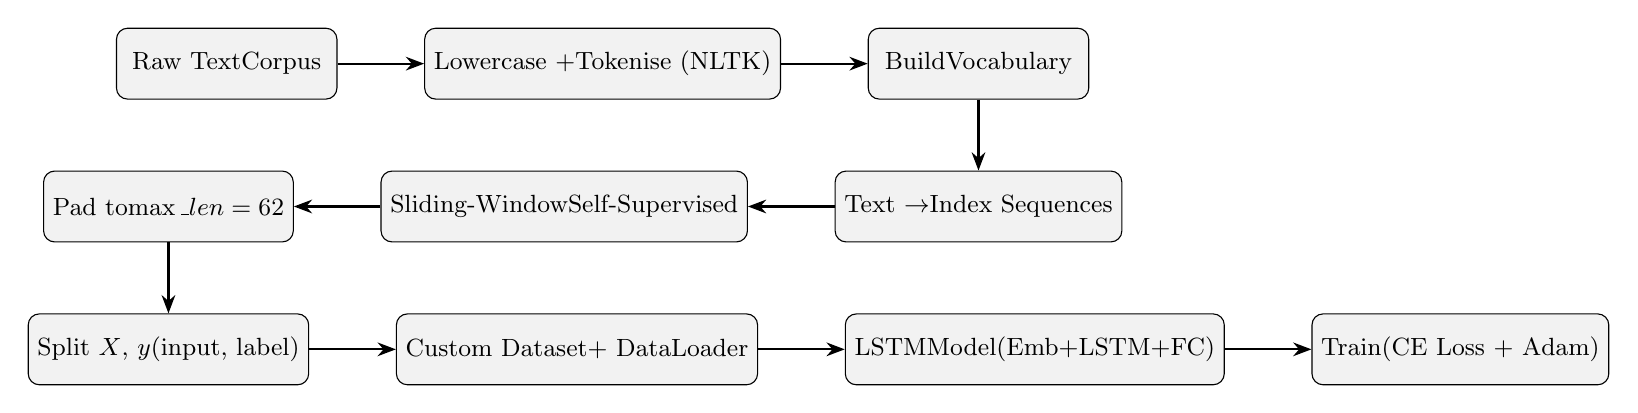
\begin{tikzpicture}[
    >=Stealth,
    node distance=0.5cm and 0.1cm,
    box/.style={draw, rounded corners=4pt, fill=gray!10,
                minimum width=2.8cm, minimum height=0.9cm,
                text centered, font=\small},
    arr/.style={->, thick}
  ]
  \node (raw)   [box]                          {Raw Text\\Corpus};
  \node (lower) [box, right=1.1cm of raw]      {Lowercase +\\Tokenise (NLTK)};
  \node (vocab) [box, right=1.1cm of lower]    {Build\\Vocabulary};
  \node (idx)   [box, below=0.9cm of vocab]    {Text $\to$\\Index Sequences};
  \node (slide) [box, left=1.1cm of idx]       {Sliding-Window\\Self-Supervised};
  \node (pad)   [box, left=1.1cm of slide]     {Pad to\\$\max\_len=62$};
  \node (split) [box, below=0.9cm of pad]      {Split $X$, $y$\\(input, label)};
  \node (data)  [box, right=1.1cm of split]    {Custom Dataset\\+ DataLoader};
  \node (model) [box, right=1.1cm of data]     {LSTMModel\\(Emb+LSTM+FC)};
  \node (train) [box, right=1.1cm of model]    {Train\\(CE Loss + Adam)};

  \draw[arr] (raw)   -- (lower);
  \draw[arr] (lower) -- (vocab);
  \draw[arr] (vocab) -- (idx);
  \draw[arr] (idx)   -- (slide);
  \draw[arr] (slide) -- (pad);
  \draw[arr] (pad)   -- (split);
  \draw[arr] (split) -- (data);
  \draw[arr] (data)  -- (model);
  \draw[arr] (model) -- (train);
\end{tikzpicture}
\caption{End-to-end pipeline for the next-word prediction hands-on
  (\texttt{pytorch-lstm-next-word-predictor.ipynb}).}
\label{fig:pipeline}
\end{figure}

\subsection{Step 1: Tokenisation and Vocabulary Construction}
\label{subsec:tokenisation}

The raw text is processed as follows:

\begin{enumerate}[label=\textbf{\arabic*.}]
  \item \textbf{Lowercase conversion.}  All characters are converted to
    lowercase so that \texttt{About} and \texttt{about} are treated as the
    same token.  Python is case-sensitive; without this step the vocabulary
    would contain duplicates.

  \item \textbf{Word tokenisation.}  NLTK's \texttt{word\_tokenize} splits
    the text into individual word tokens and punctuation, automatically
    discarding HTML-style artefacts (e.g.\ \verb|\/|).

  \item \textbf{Frequency counting.}  A \texttt{Counter} object maps each
    unique token to its frequency.  The keys of this dictionary become the
    vocabulary.

  \item \textbf{Index assignment.}  Starting from index 1 (index 0 is
    reserved for the \texttt{<UNK>} token to handle out-of-vocabulary words
    at test time), each new token receives the next integer index.
\end{enumerate}

The resulting vocabulary size is $V = 289$ unique tokens.

\subsection{Step 2: Converting Sentences to Index Sequences}
\label{subsec:index-seq}

The document is split on newline characters (\verb|\n|), yielding 78
sentences of varying length.  A helper function \texttt{text\_to\_indices}
converts each sentence from a list of string tokens to a list of integer
indices by looking up the vocabulary dictionary; unknown tokens receive
index 0.

\subsection{Step 3: Self-Supervised Sliding-Window Sequences}
\label{subsec:sliding-window}

Next-word prediction is a \emph{self-supervised} task: the supervision signal
is derived from the data itself without manual annotation.  For each sentence
of length $L$ (represented as indices $[w_1, w_2, \ldots, w_L]$), the
following training pairs are generated:

\begin{center}
\begin{tabular}{lll}
\toprule
\textbf{Input sequence $X$}   & \textbf{Target $y$} & \textbf{Interpretation} \\
\midrule
$[w_1]$                       & $w_2$               & Given first word, predict second \\
$[w_1, w_2]$                  & $w_3$               & Given first two, predict third \\
$[w_1, w_2, w_3]$             & $w_4$               & \ldots \\
$\vdots$                      & $\vdots$            & \\
$[w_1, \ldots, w_{L-1}]$      & $w_L$               & Given all but last, predict last \\
\bottomrule
\end{tabular}
\end{center}

This produces a total of 942 training sequences from the 78 sentences.
Sequence lengths vary from 2 tokens (shortest) up to 62 tokens (longest).

\begin{example}[title=Sliding-Window Output for Sentence 10]
\begin{verbatim}
training_sequence[10]
# [ [3, 7],
#   [3, 7, 5],
#   [3, 7, 5, 2],
#   [3, 7, 5, 2, 6],
#   [3, 7, 5, 2, 6, 7],
#   ... ]
\end{verbatim}
Each sub-list is one training example.  The last element of the sub-list is
the target word; everything before it is the input context.
\end{example}

\subsection{Step 4: Padding to Uniform Length}
\label{subsec:padding}

Because PyTorch processes data in \emph{batches}, all sequences within a
batch must share the same length.  The maximum sequence length found in the
dataset is 62, so all shorter sequences are left-padded with zeros:

\[
  \text{padded\_seq} = [\underbrace{0,\ldots,0}_{62-L},\; w_1,\; w_2,\; \ldots,\; w_L].
\]

Left-padding (rather than right-padding) is used so that the target word
always occupies the \emph{last} position of the padded array, enabling a
uniform \texttt{y = sequence[-1]} split.

\begin{warningbox}[title=Why Left-Pad, Not Right-Pad]
  If zeros were appended to the right, the last column of the padded matrix
  would contain zeros for all short sequences, and those zeros would become
  the prediction targets.  Training on zero-targets would teach the model to
  predict ``unknown'' at the end of every sentence --- a catastrophic failure
  of data preparation.  Left-padding avoids this entirely.
\end{warningbox}

\subsection{Step 5: Input/Label Split}
\label{subsec:xy-split}

After padding, each training example is a length-62 integer vector.  The
split is:

\begin{itemize}
  \item $X = \text{sequence}[0:61]$ (first 61 tokens) --- the input context.
  \item $y = \text{sequence}[61]$ --- the target word to predict.
\end{itemize}

This yields a dataset $X \in \mathbb{Z}^{942 \times 61}$ and
$y \in \mathbb{Z}^{942}$.

\subsection{Step 6: PyTorch Dataset and DataLoader}
\label{subsec:dataset}

A standard PyTorch \texttt{Dataset} subclass wraps $X$ and $y$, and a
\texttt{DataLoader} creates mini-batches of size 32 with shuffling:

\begin{itemize}
  \item \texttt{\_\_len\_\_}: returns 942 (total training examples).
  \item \texttt{\_\_getitem\_\_(i)}: returns $(X[i], y[i])$ as tensors.
\end{itemize}

The DataLoader draws random batches of 32 examples, so each epoch consists
of $\lceil 942 / 32 \rceil = 30$ gradient updates.

\subsection{Step 7: LSTMModel Architecture}
\label{subsec:model}

The model is implemented as a PyTorch \texttt{nn.Module} with three components
arranged in sequence:

\begin{center}
\begin{tabular}{llll}
\toprule
\textbf{Layer}          & \textbf{Class}      & \textbf{Input shape}        & \textbf{Output shape} \\
\midrule
Embedding               & \texttt{nn.Embedding}  & $(B, 61)$ indices           & $(B, 61, 100)$ \\
LSTM                    & \texttt{nn.LSTM}       & $(B, 61, 100)$              & $(B, 61, 150)$ \\
Linear (FC head)        & \texttt{nn.Linear}     & $(B, 150)$ (last step only) & $(B, 289)$ logits \\
\bottomrule
\end{tabular}
\end{center}

\begin{example}[title=LSTMModel Class (PyTorch)]
\begin{verbatim}
class LSTMModel(nn.Module):
    def __init__(self, vocab_size, embedding_dim,
                 hidden_size, num_layers=1):
        super(LSTMModel, self).__init__()
        self.embedding = nn.Embedding(vocab_size, embedding_dim)
        self.lstm = nn.LSTM(embedding_dim, hidden_size,
                            num_layers=num_layers,
                            batch_first=True)
        self.fc = nn.Linear(hidden_size, vocab_size)
        self.total_hidden_states = num_layers * hidden_size

    def forward(self, x):
        embedded = self.embedding(x)          # (B, T, d_e)
        lstm_out, (hidden_state, cell_state) \
            = self.lstm(embedded)             # (B, T, H)
        output = self.fc(lstm_out[:, -1, :])  # (B, V)
        return output

model = LSTMModel(
    vocab_size=100,
    embedding_dim=100,
    hidden_size=100,
    num_layers=1
)
\end{verbatim}
The line \texttt{lstm\_out[:, -1, :]} extracts only the hidden state at the
\emph{last} time step, which encodes the full context of the input sequence.
This single 150-dimensional vector is then projected to logits over the
289-word vocabulary.
\end{example}

\begin{keyinsight}[title=Why \texttt{batch\_first=True}?]
  By default, PyTorch's \texttt{nn.LSTM} expects input of shape
  $(T, B, d_e)$ (time first).  Setting \texttt{batch\_first=True} changes
  this to $(B, T, d_e)$ (batch first), which is more natural when indexing
  with \texttt{lstm\_out[:, -1, :]} (select all batches, last time step).
  Without this flag, the equivalent slice would be
  \texttt{lstm\_out[-1, :, :]} (last time step, all batches), which is less
  readable.
\end{keyinsight}

\subsection{Step 8: Training Loop}
\label{subsec:training}

The model is trained for 10 epochs with:
\begin{itemize}
  \item \textbf{Loss function:} Cross-entropy loss
    $\mathcal{L} = -\sum_{k=1}^{V} y_k \log \hat{p}_k$, applied to the
    vocabulary logits.
  \item \textbf{Optimiser:} Adam with learning rate $\eta = 0.01$.
  \item \textbf{Device:} GPU if available (\texttt{cuda}), else CPU.
\end{itemize}

\newpage
%% ============================================================
\section{Comparison Tables}
\label{sec:tables}
%% ============================================================

\subsection{LSTM Gate Properties}
\label{subsec:gate-table}

\begin{table}[ht]
\centering
\caption{Summary of LSTM gate properties for a single time step.}
\label{tab:gate-props}
\begin{tabularx}{\textwidth}{lXXXX}
\toprule
\textbf{Gate}    & \textbf{Equation}
                 & \textbf{Activation}
                 & \textbf{Acts on}
                 & \textbf{Role} \\
\midrule
Forget $f_t$
  & $W_{xf}x_t + W_{hf}h_{t-1} + b_f$
  & Sigmoid $\in [0,1]$
  & $C_{t-1}$
  & Decides how much old memory to erase \\[4pt]
Input $i_t$
  & $W_{xi}x_t + W_{hi}h_{t-1} + b_i$
  & Sigmoid $\in [0,1]$
  & $\tilde{C}_t$
  & Decides how much new info to write \\[4pt]
Candidate $\tilde{C}_t$
  & $W_{xC}x_t + W_{hC}h_{t-1} + b_C$
  & Tanh $\in [-1,1]$
  & (new proposal)
  & Generates candidate update values \\[4pt]
Output $o_t$
  & $W_{xo}x_t + W_{ho}h_{t-1} + b_o$
  & Sigmoid $\in [0,1]$
  & $\tanh(C_t)$
  & Filters memory for short-term output \\
\bottomrule
\end{tabularx}
\end{table}

\subsection{Hyperparameters Used in the Hands-On}
\label{subsec:hyperparams}

\begin{table}[ht]
\centering
\caption{Hyperparameter values used in the hands-on notebook.}
\label{tab:hyperparams}
\begin{tabular}{lll}
\toprule
\textbf{Hyperparameter}    & \textbf{Value} & \textbf{Notes} \\
\midrule
Vocabulary size ($V$)      & 289            & Unique tokens after lowercasing \\
Embedding dimension ($d_e$)& 100            & \texttt{nn.Embedding} output size \\
Hidden size ($H$)          & 150            & LSTM neurons per gate \\
Number of LSTM layers      & 1              & Single-layer LSTM \\
Sequence length ($T$)      & 61             & After left-padding to 62, minus label \\
Batch size                 & 32             & Mini-batch gradient descent \\
Epochs                     & 10             & Full passes over training data \\
Learning rate ($\eta$)     & 0.01           & Adam optimiser \\
Max sequence length        & 62             & Determined from training data \\
Training sequences         & 942            & Generated by sliding-window \\
Sentences in corpus        & 78             & After splitting on newlines \\
\bottomrule
\end{tabular}
\end{table}

\subsection{Forget Gate Numerical Results}
\label{subsec:forget-table}

\begin{table}[ht]
\centering
\caption{Forget gate numerical walkthrough results (4-dimensional example).}
\label{tab:forget-nums}
\begin{tabular}{ccccc}
\toprule
\textbf{Dim.} & $z_f[k]$ & $f_t[k] = \sigma(z_f[k])$ & $C_{t-1}[k]$ & $f_t[k]\cdot C_{t-1}[k]$ \\
\midrule
0 & $1.2$  & $0.77$ & $0.9$ & $0.69$ \\
1 & $-0.5$ & $0.38$ & $0.2$ & $0.08$ \\
2 & $0.3$  & $0.57$ & $0.8$ & $0.46$ \\
3 & $2.0$  & $0.88$ & $0.4$ & $0.35$ \\
\bottomrule
\end{tabular}
\end{table}

%% ============================================================
\section{Summary and Conclusions}
\label{sec:summary}
%% ============================================================

Session 20 achieved two closely linked objectives:

\paragraph{Objective 1: Demystifying LSTM Mathematics.}
By working through a complete 4-dimensional numerical example, the session
gave students a concrete, calculable understanding of how the three LSTM
gates operate.  The key equations --- \cref{eq:full-ft} through
\cref{eq:full-ht} --- were derived step by step, with each intermediate vector
explicitly computed and interpreted.  The central insight is that LSTM resolves
the vanishing gradient problem by (a) maintaining a dedicated cell-state
highway $C_t$ updated only additively, and (b) using learnable, input-dependent
gates to modulate what is forgotten, what is added, and what is exposed.

\paragraph{Objective 2: Building a Working Language Model.}
The hands-on demonstrated that the same LSTM equations, when wrapped in a
\texttt{nn.Module} with an embedding layer and a linear projection head, can
be trained end-to-end on a next-word prediction task using standard PyTorch
utilities.  All stages of the NLP pre-processing pipeline were covered:
tokenisation, vocabulary construction, self-supervised sliding-window sequence
generation, left-padding for batched processing, and dataset/dataloader setup.

\begin{keyinsight}[title=Core Takeaways from Session 20]
\begin{enumerate}[label=\arabic*.]
  \item The LSTM cell state $C_t$ is a \textbf{long-term memory highway};
    the hidden state $h_t$ is a \textbf{context-filtered short-term output}.
  \item All internal vectors ($x_t$, $h_t$, $C_t$, $f_t$, $i_t$, $o_t$,
    $\tilde{C}_t$) must share the same dimension $H$.
  \item The forget gate multiplies $C_{t-1}$ by values in $[0,1]$;
    the input gate adds a fraction of the candidate $\tilde{C}_t$.
    Together, \cref{eq:full-cell} is the only update to long-term memory.
  \item In PyTorch, \texttt{nn.LSTM} encapsulates all gate computations.
    With \texttt{batch\_first=True}, input shape is
    $(B, T, d_e)$ and \texttt{lstm\_out[:, -1, :]} gives the final-step
    hidden state for classification or prediction.
  \item Batched processing of variable-length sequences requires
    \textbf{padding}.  Left-padding ensures the true target token always
    occupies the last position, avoiding zero-target training artefacts.
\end{enumerate}
\end{keyinsight}

\paragraph{Looking Ahead.}
Session 21 will introduce the Gated Recurrent Unit (GRU), which achieves
comparable performance to LSTM with approximately 25\% fewer parameters by
merging the cell state and hidden state into a single vector and replacing
the three separate gates with just two (reset and update).

\end{document}
